\section{Cadre du projet}

\subsection{Présentation du projet}

Pour gérer la vaste gamme d'appareils de point de vente (TPE), les fournisseurs de paiements doivent mettre à niveau leurs réseaux TPE avec la dernière technologie pour prendre en charge tous les terminaux. Dans le même temps, les prestataires de paiement doivent gérer de manière proactive leurs réseaux TPE à distance, sans la présence physique d'un ingénieur. Tout cela est essentiel si les prestataires de paiement souhaitent offrir des services à valeur ajoutée.\\

Tout système de point de vente devra également piloter les appareils, switch d'autorisation, capturer les données de transaction et gérer la compensation et le règlement de manière rentable, dynamique et efficace. Enfin, le système de point de vente doit prendre en charge les technologies futures et disposer d'API ouvertes pour les appareils gérés par des tiers.\\

\begin{figure}[h!]  
  \centering
    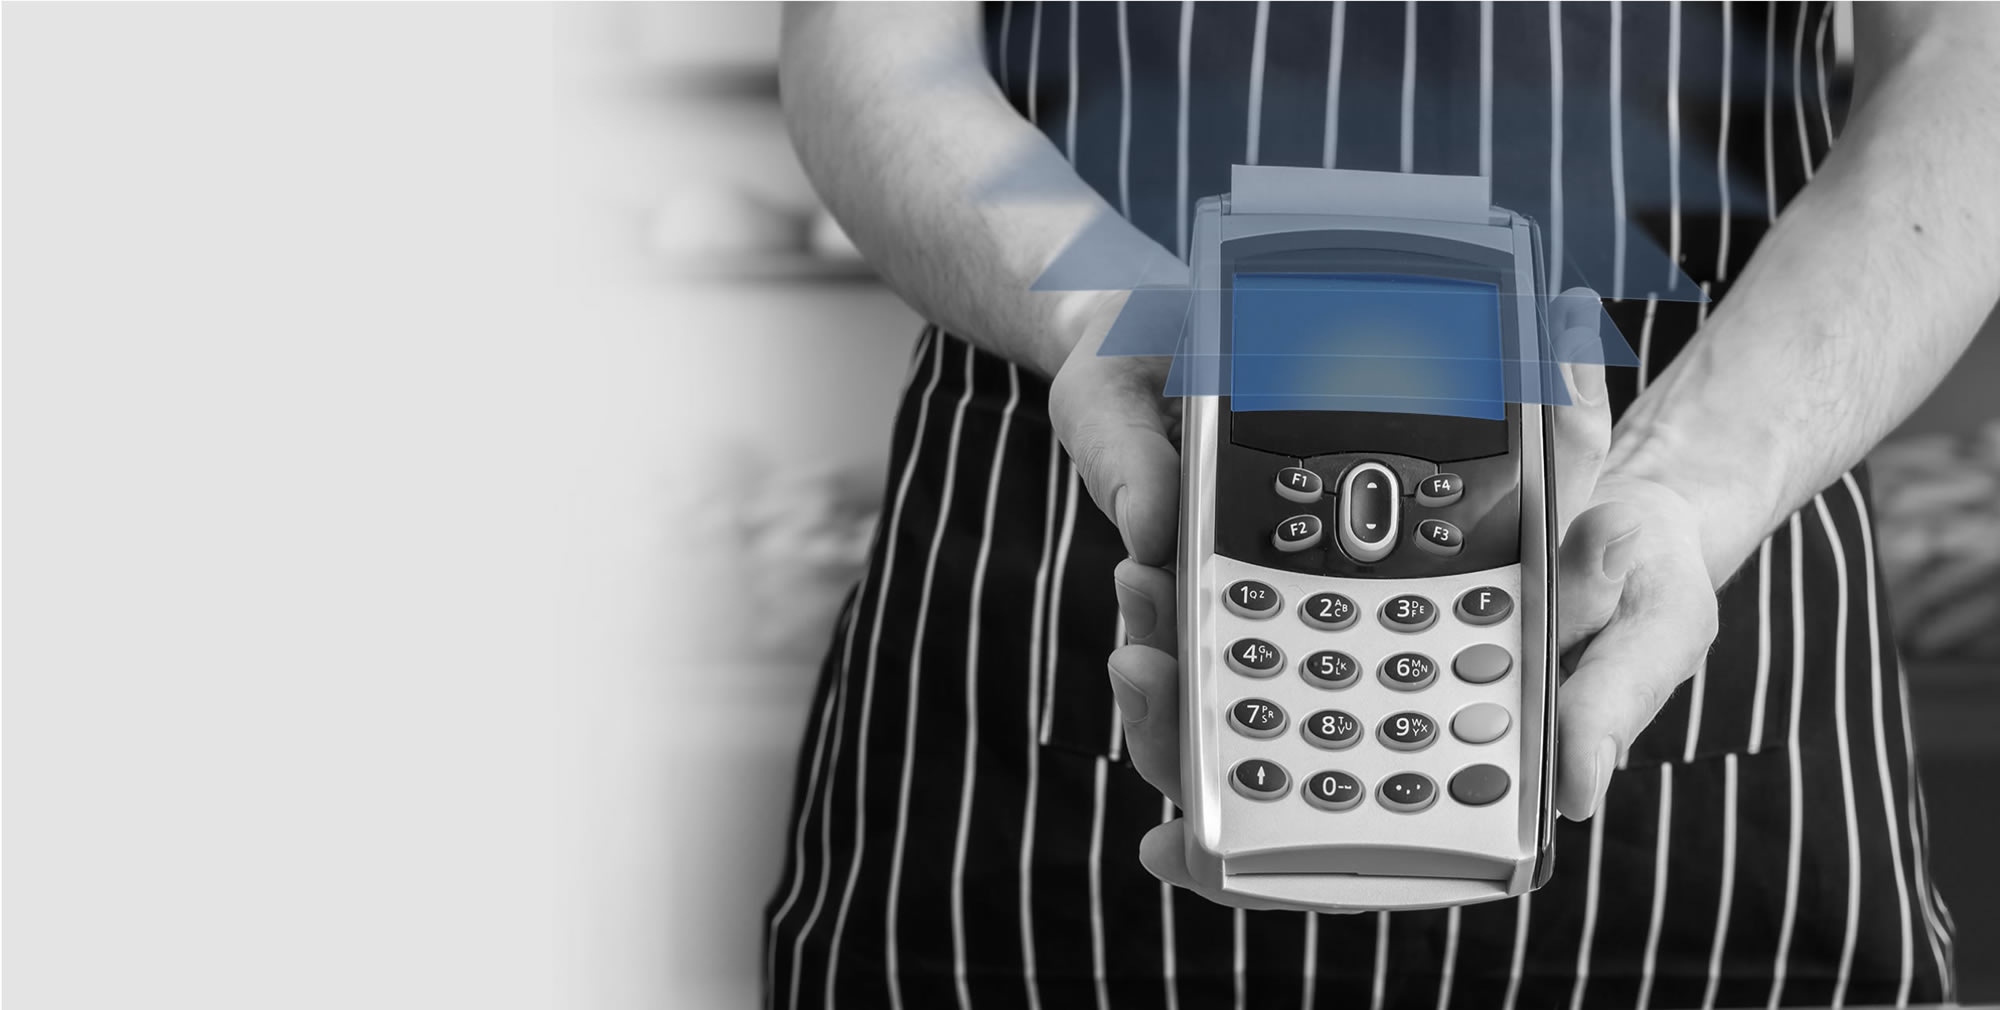
\includegraphics[width=0.7\textwidth]{chapitre1/Figures/pmo.png}
\end{figure}


C'est pour cela, une solution de monitoring des TPE s’avère indispensable, elle va permettre d'afficher informations relatives à l’état de fonctionnement de tous les TPE et la mise à disposition de statistiques relatifs  à l’activité de chaque terminal.

\subsection{Objectif du projet}
Notre projet de fin d'étude consiste à mettre en place une solution répondant aux objectifs suivant :
\begin{itemize}
\item Surveiller / maintenir l'état du terminal en temps réel
\item Surveiller les diagnostics matériels du terminal
\item Rapports et tableaux de bord
\item Surveillance et gestion des points de vente indépendants du vendeur
\item Suivi et reporting des authorizations
\item le suivi des revenus ainsi que les pertes par terminal
\end{itemize}

\subsection{Besoins du projet}

\subsubsection{Exigences fonctionnelles}

Pour répondre à un besoin réel, en termes de contraintes fonctionnelles, l'application doit permettre aux utilisateurs plusieurs fonctionnalités présentées comme suit :
\begin{itemize}
\item Module de paramétrage : ce module permet de définir les paramètres de l'application (status des composants, les composants du terminal,  ...)
\item Module opération : ce module permet le monitoring des terminaux (état des composants, le suivi des revenus, les statistiques liées aux autorisations, ...) 
\end{itemize}

\subsubsection{Exigences techniques}

Le système doit répondre aux exigences techniques suivantes :
\begin{itemize}
\item Déploiement : L’application devra être déployée sur un serveur d'application.  Le serveur sera configuré pour fonctionner en mode sécurisé et servira comme serveur frontal.
\item Convivialité de l’interface : respect des règles adoptées par HPS pour toutes ses applications.
\end{itemize}

\subsubsection{Exigences non fonctionnelles}

En ce qui concerne les objectifs en termes qualité, le système doit répondre autant que possible aux exigences suivantes : 
\begin{itemize}
\item Fiabilité : Le système doit fonctionner sans défaillance pour une durée donnée (robuste, constant, etc…)
\item Efficacité : Le système doit fonctionner avec un optimum de ressources et de temps
\item Testabilité : Le système doit être facilement testable pour s'assurer de son bon fonctionnement (jeu d'essais et vérification de résultats)
\item Sécurité : L’application  doit  assurer  un  système  de  sécurité  flexible,  permettant  d’accéder aux fonctionnalités du système selon les droits et les rôles de l'utilisateur
\item Facilité d’utilisation : Le système doit offrir une facilité pour l'apprentissage et le dialogue Homme/machine (compréhensible, maniable, documentation, etc.…)
\end{itemize}
